\section{INTRODUCTION} \label{intro}

Since its rise, deep learning had a great impact on discriminative models. Generative models instead were not affected by this innovation at first, but this trend changed with the introduction of Generative Adversarial Networks (GAN), a powerful framework first introduced in \cite{NIPS2014_5423}. Since then, GAN gained more and more momentum because of the ability of training \textit{deep generative models}, avoiding some of the difficulties encountered in other frameworks \cite{DBLP:journals/corr/Goodfellow17}.

GAN is a sub-class of generative models where a probability density function (pdf) is implicitly defined; since GAN makes use of, generally two, \textit{neural networks}, the pdf is induced by their architecture and parameters design: given a training set of sample data, distributed according to an unknown pdf $p_{data}$, the purpose of GAN is indeed to generate samples according to a distribution $p_g$, that mimics $p_{data}$, without explicitly defining it.
As suggested by the name, this is achieved by putting in competition two entities: a generator and a discriminator. The task of the generator (G) is to generate data that can be regarded as true by the discriminator, while the discriminator (D) has the purpose of correctly distinguishing real from fake data. The classical real-life analogy with this process involves counterfeiters trying to produce fake currency and the police trying to detect it. A graphical representation of the process is depicted in fig.\ref{fig:game}.
This kind of interaction between the two entities can naturally be modeled with a game theoretical approach, where each player has its own strategies and payoffs, but in this paper we will rather talk about costs, as will be discussed in \ref{relatedwork}. The major drawback of this framework anyway, is that the training of the model requires to compute the Nash Equilibrium (NE) of the game involving the two entities, which is not as simple as optimizing an objective function: without the guarantee of a NE, results obtained by the model could be different fom the ones desired.

In this paper we review some of the literature and explain our need to go back to the origins of GAN, implementing our own version of the code and simulating different scenarios, where discriminator is passed different fake-to-true ratios of images.

The remainder of the paper is organized as follows: a brief overview of the literature is presented in \ref{relatedwork}; a description of our work is then presented in \ref{expsetting}; the obtained results are presented in \ref{results}; finally we discuss our conlcusions in \ref{conclusions}.


\begin{figure}
	\begin{center}
		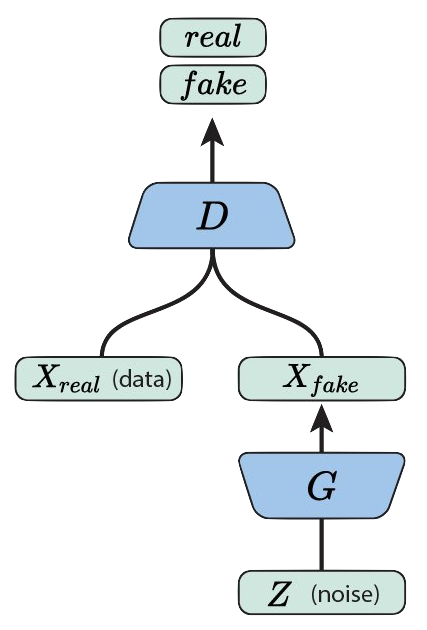
\includegraphics[scale=0.25]{./plots/GAN_model.png}
	\end{center}
	\caption{a block-diagram representing generative adversarial networks. A generator network (G) creates samples in data space from noise. A discriminator network then compares data, trying to distinguish true from fake samples.}
	\label{fig:game}
\end{figure}